% This file contains only the fully dressed use cases
\label{useCases}

\subsection{Preface}

Users will have instant access to the functionality of the site as soon as they
have created an account and logged in. That is, they can perform all of the functions
that an investor can perform. They will also have the ability to choose to create or
join a league, though they are not required to in order to experience the full
functionality of the software. This will give our software a broader demographic
when compared to that of years prior. That being said, league creation and
administrative user delegation will be an important part of the functionality of
the program and will be described its own use case. Core functionalities of respect
user types will be elaborated below.\\

\subsection{Fully-Dressed Use Cases}

Having an account within our database is necessary for the user to experience
functionality within the software. That being said, the user can create an account in
different ways. They can choose to have the information imported by logging in through
any OpenID/OAuth service service (eg: google, facebook, twitter, etc.) This will populate
the database fields automatically with data driven from the external resources.
Once the user has created an account, they can log in through OpenID/OAuth and will
generally remain logged into the system as long as they remain logged into their service
of their choice.\\

\textbf{CG-BP01} – A user can create an account such to access the full features of the game.
They can return and log in with minimal burden and access all of the information previously
stored. \\

\begin{centering}
\renewcommand\arraystretch{1.3} % Causes rows to be spaced
\label{UC-1}
\begin{longtable}{|p{1.2in} p{5in}|}

\hline
\bfseries{\color{color1}Use Case UC-1} &
\bfseries{\color{color1}Register/Create an account using OpenID/OAuth2} \\
\hline
Related Requirements: & ST-1, ST-2 \\
Initiating Actor:     & Guest \\
Actor's Goal:         & Register with our servers\\
Participating Actors: & Guest, Database\\
Preconditions:        & -Guest must not be a registered user\\
Postconditions:       & -The \textbf{Database} is updated with guests information and
                         logs the guess in as an \textbf{Investor}\\
\hline
\multicolumn{2}{|c|}{\color{color1}Flow of Events for Main Success Scenario:}\\
\hline
$\rightarrow$ & 1. \textbf{Guest} navigates to Paramount Investment League and logs in \\
 $\leftarrow$ & 2. \textbf{System} checks \textbf{database} for \textbf{investor} and
isn't found\\
 $\leftarrow$ & 3. \textbf{System} retrieves OpenID/OAuth info and registers guest
in \textbf{database} as an \textbf{investor}\\
$\rightarrow$ & 4. \textbf{System} sends out confimation to user and displays starter
portfolio \\
\hline
\multicolumn{2}{|c|}{\color{color1}Flow of Events for Alternate Scenarios:} \\
\hline
$\rightarrow$ & 1.  \textbf{Investor} attempts to login  \\
 $\leftarrow$ & 2. \textbf{System} checks \textbf{Database} and finds \textbf{investor}\\
 $\leftarrow$ & 3. \textbf{System} loads \textbf{investor} info from \textbf{database} \\
$\rightarrow$ & 4. \textbf{System} displays users portfolio \\
\hline
\end{longtable}
\end{centering}

Any user has the option at any time to create or join a league. The user who has requested
to create a league will have elevated privileges versus a standard user. The league manager
will be prompted to make a league with various setting options for victory condition, badges,
achievements, etc. The league manager can also choose whether or not to make the league private.
A private league will restrict users to those invited by the league manager, and will require
a password to join. After initial setup, league managers will have minimal access to settings.
That is, halfway through a league, the manager cannot decide to change the victory conditions.
This prevents the league manager from abusing power to tip the scales in his or her favor.\\

\textbf{CG-BP02} – A user can create a league or join a league if he or she desires. Note that
users may trade without a league, but has access to create or join a new league at any time.
Leagues may be private or public. \\


\begin{centering}
\renewcommand\arraystretch{1.3}
\label{UC-2}
\begin{longtable}{|p{1.2in} p{5in}|}
\hline
\bfseries{\color{color1}Use Case UC-2} &
\bfseries{\color{color1}Create/Join a League} \\
\hline
Related Requirements: & ST-3, ST-8, ST-16, ST-17, ST-18\\
Initiating Actor:     & Investor \\
Actor's Goal:         & Create or join a league to compete in\\
Participating Actors: & Database, other Investors \\
Preconditions:        & -Investor is logged in \\
                      & -league is not created or user hasn't joined league \\
Postconditions:       & -The league is created with the appropriate settings or \\
                      & -The \textbf{Investor} has joined the league \\
                      & -The \textbf{Database} has been updated \\
\hline
\multicolumn{2}{|c|}{\color{color1}Flow of Events for Main Success Scenario:}\\
\hline

$\rightarrow$ & 1. \textbf{Investor} navigates to and clicks on the create league dialogue. \\
$\rightarrow$ & 2. \textbf{System} displays to the \textbf{Investor} the available options for
creating a league.  \\
$\rightarrow$ & 3. \textbf{Investor} updates the settings, such as privacy, league name, number of spots, and managing users \\
$\leftarrow$ & 4. \textbf{System} sends the updated settings to the \textbf{Database} \\
$\rightarrow$ & 5. \textbf{System} sends confimation to the \textbf{Investor} \\
\hline

\multicolumn{2}{|c|}{\color{color1}Flow of Events for Alternate Scenarios:} \\
\hline

\multicolumn{2}{|p{6.2in}|}{3a. The \textbf{Investor} selects league settings that are disallowed,
such as a league name that already exists.} \\ \hline

$\rightarrow$ & 4. \textbf{System} informs user what settings are incorrect.\\ \hline

\multicolumn{2}{|p{6.2in}|}{\textbf{Investor} wishes to join a league} \\
\hline

$\rightarrow$ & 1. \textbf{Investor} navigates to league listing.\\
$\leftarrow$ & 2. \textbf{System} updates \textbf{database} with \textbf{investors} info.\\
$\rightarrow$ & 3. \textbf{System} confirms \textbf{investor} as part of league and displays
league site.\\
\hline
\end{longtable}
\end{centering}

Users can view raw market data which will be pulled from Yahoo Finance in near real time.
Users can view company data either on their own portfolio page or through the company’s
specific info page. That is, the user can view detailed information of each stock or company
before committing to a trade from a variety of sources. Users will be able to compare their
portfolio’s performance to typical market trends from the Nasdaq, S\&P 500, and DJIA. There
will also be a stock ticker ribbon on the bottom of the screen for users to receive constant
real time feeds of most recent trades happening within the market.\\

\textbf{CG-BP03} – A user can view market data in near-real time. They will have access to data
taken from the Yahoo! Finance API and can view this data in their portfolio or by searching
for stocks using tickers. \\

\begin{centering}
\renewcommand\arraystretch{1.3}
\label{UC-3}
\begin{longtable}{|p{1.2in} p{5in}|}
\hline
\bfseries{\color{color1}Use Case UC-3} &
\bfseries{\color{color1}View Market Data} \\
\hline
Related Requirements: & ST-4, ST-5, ST-10, ST-11 \\
Initiating Actor:     & Investor \\
Actor's Goal:         & View the latest information about stocks, companies, and trades\\
Participating Actors: & Database, Yahoo! Finance \\
Preconditions:        & -Yahoo! Finance is accepting inquiries \\
                      & -Investor is logged in \\
Postconditions:       & -None worth mentioning \\

\hline
\multicolumn{2}{|c|}{\color{color1}Flow of Events for Main Success Scenario:}\\
\hline

$\rightarrow$ & 1. \textbf{Investor} searches for a market term  \\
 $\leftarrow$ & 2. \textbf{System} sends request to \textbf{database} \\
$\rightarrow$ & 3. \textbf{System} returns suggested terms \\
$\rightarrow$ & 4. \textbf{Investor} selects a term from suggested terms list and sends request \\
$\leftarrow$ & 5. \textbf{System} sends request to \textbf{Yahoo! Finance} \\
$\leftarrow$ & 6. \textbf{database} is updated. \\
\hline

\multicolumn{2}{|c|}{\color{color1}Flow of Events for Alternate Scenarios:} \\
\hline

\multicolumn{2}{|p{6.2in}|}{Search Fails} \\
\hline

$\leftarrow$ & 6. \textbf{Yahoo! Finance} returns no results \\
$\rightarrow$ & 7. \textbf{System} informs \textbf{investor} of search failure \\

\hline

\end{longtable}
\end{centering}

User will be able to view all major items within their portfolio as well as place trades from
their portfolio page. From this page, a user can view detailed analysis and graphs of each
of their respective stocks as well as their current rank within their league (if applicable)
and globally. Users will also be able to place trades for respective companies through their
portfolio page. Users can buy, sell, short, or carry out any additional action on any stock
or security within the limits of their finances and league settings through this page (See UC-5).
Users will also be able to customize and change views as well as add stock index comparisons
to monitor their success vs market success.\\

\textbf{CG-BP04} – All users will have a portfolio which will house detailed information
regarding all of their stocks and performance. They will be able to perform trades
from this location and will also have access to the core functionality of the site
through this page. It will essentially be the user’s home page. \\

\begin{centering}
\label{UC-4}
\renewcommand\arraystretch{1.3}
\begin{longtable}{|p{1.2in} p{5in}|}
\hline
\bfseries{\color{color1}Use Case UC-4} &
\bfseries{\color{color1}Manage Portfolio} \\
\hline
Related Requirements: & ST-8, ST-9, ST-10, ST-12, ST-13, ST-14 \\
Initiating Actor:     & Investor \\
Actor's Goal:         & Manage portfolio by viewing current standings/stocks/securities \\
Participating Actors: & Database, Yahoo! Finance \\
Preconditions:        & -Yahoo! Finance is accepting inquiries \\
                      & -User is logged in \\
Postconditions:       & -\textbf{Investor}'s portfolio is updated to reflect change
                        in position \\
\hline
\multicolumn{2}{|c|}{\color{color1}Flow of Events for Main Success Scenario:}\\
\hline

$\rightarrow$ & 1. \textbf{Investor} navigates to their portfolio \\
 $\leftarrow$ & 2. \textbf{System} requests users portfolio from \textbf{database}\\
$\rightarrow$ & 3. \textbf{System} displays portfolio to \textbf{investor} \\
$\rightarrow$ & 4. \textbf{Investor} adjusts their portfolio \\
 $\leftarrow$ & 5. \textbf{System} updates the \textbf{database} \\
 $\rightarrow$ & 6. \textbf{System} displays confirmation of portfolio update \\
\hline

\end{longtable}
\end{centering}

User should be able to place trades from various locations. That is, they may place it through
their portfolio by typing in the ticker and quantity of shares. They may also navigate to a
certain company’s page and elect to purchase shares there. Selling shares should be done
through the user’s portfolio where they may see the exact quantity of shares of each respective
companies they own. Error messages will be thrown and orders not processed should a user request
to buy more shares of a company the he or she can afford or the user attempts to sell more than
he or she has. Main transactions will occur through the user’s portfolio. \\

\textbf{CG-BP05} – A user can place any market order he or she wishes to place (I.E. buy,
sell, short, limit, stop, etc). These trades can be executed from multiple locations and
at the prohibitions of the league rules. \\

\begin{centering}
\label{UC-5}
\renewcommand\arraystretch{1.3}
\begin{longtable}{|p{1.2in} p{5in}|}
\hline
\bfseries{\color{color1}Use Case UC-5} &
\bfseries{\color{color1}Place a Market Order} \\
\hline
Related Requirements: & ST-6, ST-11 \\
Initiating Actor:     & Investor \\
Actor's Goal:         & Place orders to buy/sell/short stocks, or place a stop/limit order \\
Participating Actors: & Database, Yahoo! Finance API \\
Preconditions:        & -Investor is logged in \\
                      & -Yahoo! Finance is accepting inquiries \\
Postconditions:       & -\textbf{Database} us updated with the users position \\
\hline
\multicolumn{2}{|c|}{\color{color1}Flow of Events for Main Success Scenario:}\\
\hline

$\rightarrow$ & 1. \textbf{Investor} enters a market order \\
$\leftarrow$ & 2. \textbf{System} attempts to get update from \textbf{Yahoo! Finance} \\
$\leftarrow$ & 3. \textbf{System} receives information back from \textbf{Yahoo! Finance} \\
$\leftarrow$ & 4. \textbf{System} validates and records trade in \textbf{database} \\
$\rightarrow$ & 5. \textbf{System} confirms trades and displays changes in \textbf{investor}
portfolio\\
\hline

\multicolumn{2}{|c|}{\color{color1}Flow of Events for Alternate Scenarios:} \\
\hline

\multicolumn{2}{|p{6.2in}|}{3a. \textbf{System} doesn't recieve information back from
\textbf{Yahoo! Finance}} \\
\hline

$\leftarrow$ & 4. \textbf{System} notifies \textbf{investor} of failed request \\
\hline

\end{longtable}
\end{centering}

Of the 3 user types, administrator is the highest and reserved only for developers and
administrators of the software. Administrators have the ability to modify or delete leagues
or specific users if the administrator feels that power is being abused. The administrator
will also have elevated privileges to makes changes to the site. Their main purpose will be to
suspend or ban users or leagues and ensure that the site is not being abused. This includes but
is not limited to robot or AI users or user account spamming or advertising rather than trading
properly. \\

\textbf{CG-BP06} – Administrators will have access to suspend, ban, or remove leagues or players
completely. Administrators will have elevated privileges relative to other users and will
use these privileges with the sole intention of maintaining the integrity of the software.\\


\begin{centering}
\renewcommand\arraystretch{1.3} % Causes rows to be spaced
\label{UC-6}
\begin{longtable}{|p{1.2in} p{5in}|}
\hline
\bfseries{\color{color1}Use Case UC-6} &
\bfseries{\color{color1}Take Administrative Actions} \\
\hline
Related Requirements: & ST-19, ST-20, ST-21 \\
Initiating Actor:     & Site Administrator \\
Actor's Goal:         & Perform administrative work for the website, manage database \\
Participating Actors: & Database, Investors, League Manager \\
Preconditions:        & -User is the site Administrator \\
                      & -Administrative actions need to be taken \\
Postconditions:       & -Conflicts/Issues have been resolved \\
\hline
\multicolumn{2}{|c|}{\color{color1}Flow of Events for Main Success Scenario:}\\
\hline

$\rightarrow$ & 1. \textbf{Site Administrator} requests logs from \textbf{system} \\
$\leftarrow$ & 2. \textbf{System} closes saves log file and returns log report \\
\hline

\end{longtable}
\end{centering}

Depending on the specific role of the user. (I.e. investor, league manager), users should be
able to customize several different items. That is, the league manager will have ultimate
customization of the rules of his or her league, including but not limited to: victory
conditions, achievements, and starting capital. These rules are to be established prior to
the beginning of the league and not touched for the duration. League manager will also have a
few other elevated privileges depending on whether he or she also falls into the investor role
as well. Investors will be allowed to manage their own personal settings including but not
limited to: email alerts, social media integration, and notifications.\\

\textbf{CG-BP07} – League managers will have access to a list of settings which they may
select before the initiation of the league competition. They will have slightly elevated
privileges from basic investors, but not enough to abuse power. \\

\begin{centering}
\renewcommand\arraystretch{1.3} % Causes rows to be spaced
\label{UC-7}
\begin{longtable}{|p{1.2in} p{5in}|}
\hline
\bfseries{\color{color1}Use Case UC-7} &
\bfseries{\color{color1}Manage League Settings} \\
\hline
Related Requirements: & ST-16, ST-17, ST-18 \\
Initiating Actor:     & League Manager \\
Actor's Goal:         & Change league settings to the League Mangers preference \\
Participating Actors: & Database, other Investors \\
Preconditions:        & -Initiating actor is the \textbf{League Manager} \\
                      & -There are outstanding abuse reports \\
Postconditions:       & -The \textbf{Database} is updated to reflect the chagnes made. \\
 & The abuse report shows that it has been resolved on the administration page\\
\hline
\multicolumn{2}{|c|}{\color{color1}Flow of Events for Main Success Scenario:}\\
\hline

$\rightarrow$ & 1. \textbf{League Manager} makes adjustment to league settings \\
$\leftarrow$ & 2. \textbf{System} makes a update to the \textbf{Database} \\
$\rightarrow$ & 3. \textbf{System} displays updated settings to the \textbf{league manager} \\
\hline

\end{longtable}
\end{centering}

\subsection{Traceability Matrix}

The traceability matrix presented in \em Figure 3.2 \em is based on only the full
dressed use cases above and thus is only a partial representation of the complete project.\\

\begin{figure}
\centering
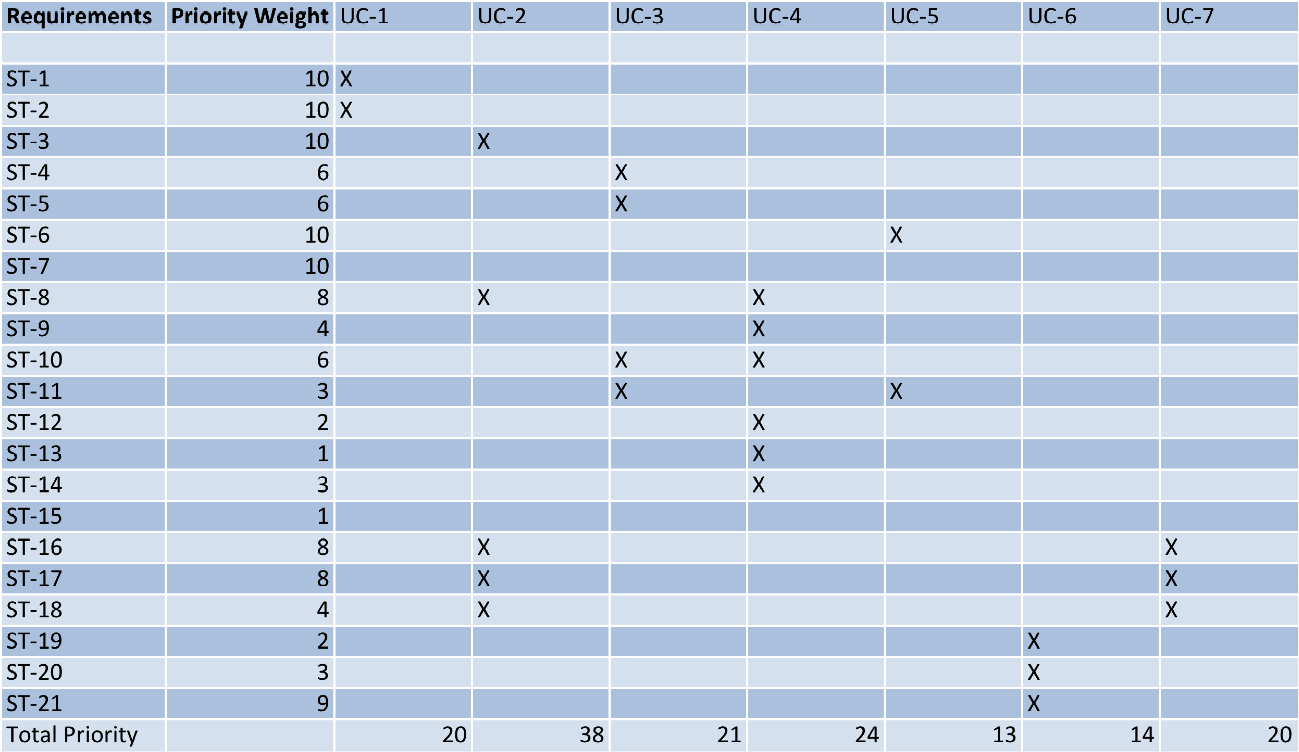
\includegraphics[width=5.5in]{./img/traceability.png}
\caption{The traceability matrix for the given use cases.}
\end{figure}

